% Generated by scripts/md_to_latex.py from paper_body.md + paper_supplementary.md.
% Do not edit by hand: change the markdown (which verify_draft.py checks) and regenerate.
\documentclass[11pt]{article}

% the PDF info dict otherwise carries the build time with the author's UTC offset
% and a banner naming the TeX distribution; the paper has no author line, so neither
\pdfinfoomitdate=1
\pdftrailerid{}
\pdfsuppressptexinfo=-1

\usepackage[margin=1in]{geometry}
\usepackage[T1]{fontenc}
\usepackage{lmodern}
\usepackage{amsmath,amssymb}
\usepackage{graphicx}
\usepackage{booktabs}
\usepackage{array}  % >{...} column specs
\usepackage[round]{natbib}
\usepackage{url}
\usepackage[hidelinks]{hyperref}
\setlength{\emergencystretch}{1.5em}  % lets lines with long numeric tokens break

\title{Knowledge the Network Already Has: An Exogeneity Precondition for Neuro-Symbolic Intrusion Detection}
\author{}
\date{}

\begin{document}
\maketitle

\begin{abstract}
Neuro-symbolic intrusion detectors that report gains from injected knowledge tend to share a property that is rarely stated: the knowledge they add, whether an asset inventory, a relational graph or an external attack taxonomy, is information the neural network could not compute from its input. Our own system did not have this property. Its Logic Tensor Network axioms are deterministic functions of the flow features the network already receives. On its own the symbolic component had no measurable effect ($-$0.0004, n.s.), and it was worse than the same trainer run without axioms in all 17 CNN training runs we paired it with, alone and combined with a knowledge-graph channel. We argue that symbolic knowledge can help a neural detector only to the extent that it lies outside the model's learned feature basis, and that the same condition explains a second failure. A closed-set classifier reaches an attack family it has never seen only in so far as that family's signature overlaps the features it learned. For Bot there is no overlap (0 of 8 discriminative features are shared), every Bot flow is classified as benign, and the ranking of Bot flows changes arbitrarily from one training seed to the next ($\rho$ = $-$0.090). The result held under five attempts to overturn it, among them an independent capture in which Bot is common and a relabelled release of the dataset. We then tried to build knowledge on CIC-IDS2017 that meets the precondition and could not. Host-role predicates derived from metadata the network never sees can still be predicted from its features, with AUC 0.990--0.994. Knowledge aggregated from the capture itself is not exogenous, and a benchmark with no external knowledge source therefore cannot support the experiment that published neuro-symbolic gains rely on.
\end{abstract}

\section{Introduction}\label{sec:1}

A common argument for neuro-symbolic learning is that domain knowledge written as logic can make up for what the training data lacks. Intrusion detection looks like a good place to test this. A data-driven detector is weakest on attacks that never appeared in training, and those are the cases where knowledge about how networks and attacks behave should matter most.

We built a neuro-symbolic intrusion detector to test the idea, and it did not work. Its Logic Tensor Network axioms encode behaviours such as burst traffic, packet-size variance and destination ports outside the standard service ports. Alone they changed macro zero-day PR-AUC by $-$0.0004, which is not significant. Compared with the same trainer run without axioms, they made the system worse with every one of the 17 CNN training runs we paired them with, whether or not a knowledge-graph channel was added. This paper sets out to explain that outcome, and we think the explanation applies beyond our system.

Published systems that do report gains have something ours did not. \citet{grov2024} add a single axiom stating that flows which do not involve a web server cannot be web attacks, and roughly double their web-attack precision. KnowGraph \citep{zhou2024} reasons over relations between entities and raises the true-positive rate from 0.0 \% to 35.5 \% at a 0.5 \% false-positive rate, a setting in which the neural baseline detects nothing. \citet{kalutharage2025} map alerts onto an external attack taxonomy. In all three, the added knowledge is something the network could not have worked out from its own input. Each of our behaviour predicates, in contrast, is a fixed function of flow features the network already reads, so at most it could act as an inductive bias. It could not add evidence.

We state this as a precondition: symbolic knowledge helps a neural detector to the extent that it lies outside the model's learned feature basis. The paper makes three contributions around it.

\begin{enumerate}
  \item \textbf{One principle with two consequences (Sections~\ref{sec:3}--\ref{sec:4}).} The same condition governs attack families that are absent from training. A closed-set learner reaches such a family only as far as the family's signature overlaps the features the learner selected. Knowledge that falls inside that basis adds nothing, and a class that falls outside it is not reached.
  \item \textbf{A durability test (Section~\ref{sec:5}).} The unreachability survives five separate attempts to break it: a capture in which the family is plentiful, corrected labels, an explicitly trained reject class, cross-dataset augmentation, and a sweep over architectures and out-of-distribution scorers.
  \item \textbf{A negative result on evaluability (Section~\ref{sec:6}).} Host-role knowledge built from metadata that the network never sees can still be recovered from the network's features. A benchmark without an external knowledge artefact cannot host the experiment on which published neuro-symbolic gains depend.
\end{enumerate}

\begin{figure}[htbp]
\centering
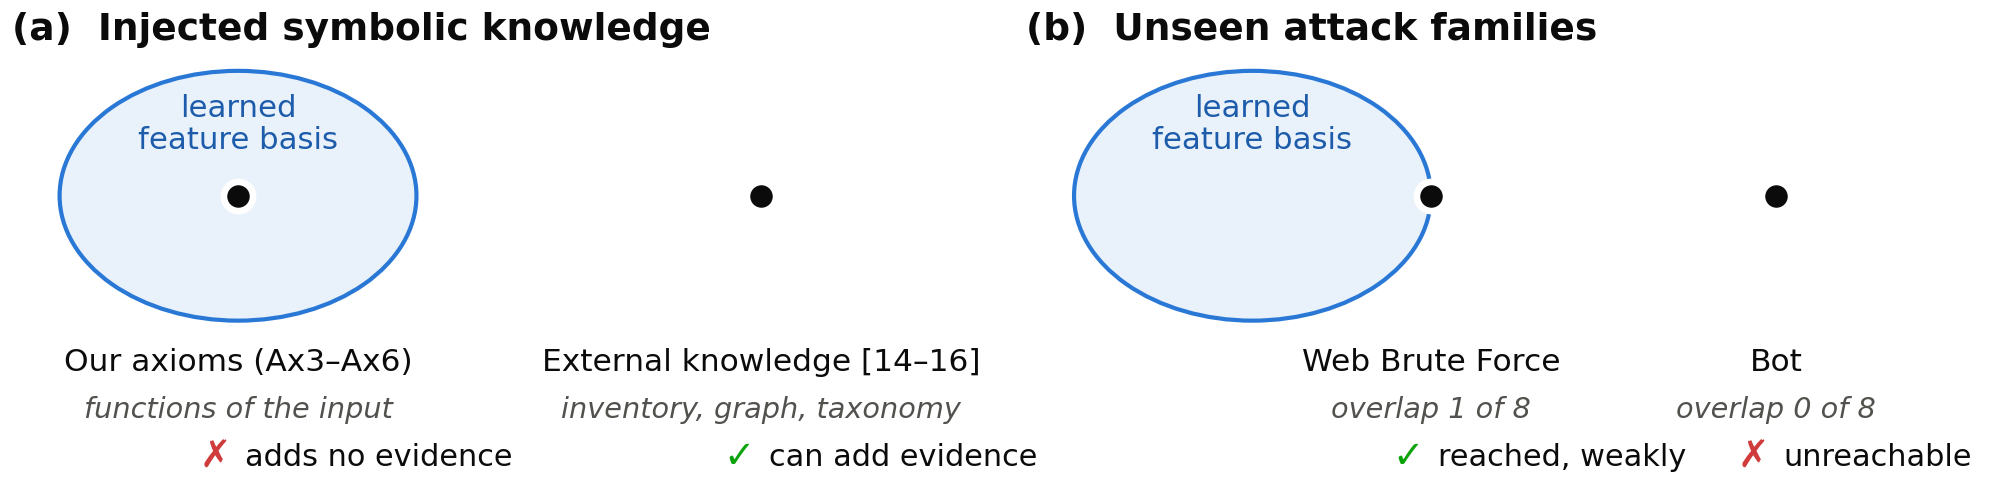
\includegraphics[width=\linewidth]{figures/nesy_fig1_thesis}
\caption{\emph{One principle, two consequences.} Both panels show the same learned feature basis, that is, the features a closed-set objective selects. (a) Symbolic knowledge can only help from outside the basis. Our Logic Tensor Network axioms are functions of the flow features and add no evidence, while the knowledge used in published systems \citep{grov2024,zhou2024,kalutharage2025} cannot be computed from the input. (b) An unseen attack family can be reached only as far as it overlaps the basis. Web Brute Force shares 1 of 8 discriminative features and is reached only weakly once label artefacts are removed (Section~\ref{sec:7}). Bot shares none and is not reached. Note that inside and outside lead to opposite outcomes in the two panels.}\label{fig:thesis}
\end{figure}

Two measurement problems limit the magnitudes we can report (Section~\ref{sec:7}), and we show both on our own system. The metric most papers report cannot separate methods by zero-day ability. In addition, once the labels are corrected, two of our three main zero-day families turn out to have been measuring whether the dataset labels a failed connection attempt as an attack. These problems cap what we can claim about effect sizes, but they do not affect the mechanism.

\section{Setting and measurement}\label{sec:2}

\textbf{Data.} We use the CIC-IDS2017 \citep{sharafaldin2018} flow features, 68 numeric features per flow. Nine attack families and benign traffic are treated as known. They are split 80/10/10 with stratification, and benign traffic is under-sampled to a 1:1 ratio, giving 883,796 training, 110,475 validation and 114,658 test flows. Six rare families (Bot, Heartbleed, Infiltration, and Web Attack Brute Force, XSS and SQL Injection) occur only in the test set.

\textbf{Metric.} Our main metric is macro zero-day PR-AUC over the three unseen families with enough samples: Bot (n = 1,956), Web Attack Brute Force (n = 1,507) and Web Attack XSS (n = 652). Heartbleed (n = 11), Infiltration (n = 36) and SQL Injection (n = 21) are too small and are left out. PR-AUC cannot fall below the prevalence of the positive class, so when test sets differ in prevalence (between datasets or between labellings) we compare lift, defined as PR-AUC divided by prevalence. A random ranker has a lift of 1.0.

\textbf{Reproducibility.} Without determinism flags, training at a fixed seed does not give identical results, so we measured run-to-run variation before comparing any methods. The standard deviation is 0.0222 from nondeterminism alone, 0.0171 across seeds with determinism enabled (n = 6) and 0.0228 across data splits, which puts the uncertainty on a single absolute number at about 0.0285. All comparisons are paired on seed. We call a difference established only if its sign is the same on every seed, and we give magnitudes as ranges. This procedure led us to withdraw one of our own earlier claims: a gap of 0.9 SD that a paired bootstrap had reported as significant (p = 0.001; Appendix~\ref{apd:E}).

\section{A symbolic pillar that could not help}\label{sec:3}

\textbf{Architecture.} The system has three parts: a 1D CNN over the flow features, a Logic Tensor Network \citep{badreddine2022} layer that grounds fuzzy axioms in network behaviours, and a knowledge-graph channel that scores how quickly clusters of flows grow over time. The axioms (Ax3--Ax6) tie the network's attack output to behaviour predicates such as large packets with high size variance, bursts, scan-like probing and a destination port outside a list of standard service ports (\texttt{BeaconLike}).

\textbf{Results.} We tried injecting the axioms at the loss, at the representation and at inference. In every case the symbolic component either lowered macro zero-day PR-AUC or left it unchanged. On its own it contributes $-$0.0004 (n.s.). The cleaner test holds everything but the axioms fixed: the same trainer with the axiom weight at zero. Against it, the axioms lower macro zero-day PR-AUC with each of the 11 CNN runs trained before our determinism controls (by 0.0062 on average) and each of the 6 trained after (0.0068), and by more when a knowledge-graph channel is also fused (0.0212 and 0.0324). An earlier version of this comparison, which added the axioms on top of a knowledge-graph fusion built on three CNN runs, reported a significant loss; that fusion does not hold across CNN runs (Appendix~\ref{apd:D}), so we report the matched comparison instead. One axiom seemed at first to help on Bot, but the effect disappeared when we repeated the experiment over several seeds. Because the sign of the effect is the same in every configuration, we do not think better tuning would change the conclusion.

Comparing our system with published ones that report gains suggests why:

\begin{center}\small
\begin{tabular}{@{}>{\raggedright\arraybackslash}p{\dimexpr 0.220\linewidth-2\tabcolsep\relax}>{\raggedright\arraybackslash}p{\dimexpr 0.455\linewidth-2\tabcolsep\relax}>{\raggedright\arraybackslash}p{\dimexpr 0.325\linewidth-2\tabcolsep\relax}@{}}
\toprule
\textbf{system} & \textbf{knowledge injected} & \textbf{computable from the flow features?} \\
\midrule
\citet{grov2024} & flows not involving a web server are not web attacks & no, needs an asset inventory \\
KnowGraph \citep{zhou2024} & logic over relations between entities & no, needs a relational graph \\
\citet{kalutharage2025} & mapping of techniques to an attack taxonomy & no, needs an external taxonomy \\
ours & behaviour predicates (Ax3--Ax6) & yes, each is a function of the input \\
\bottomrule
\end{tabular}
\end{center}

All seven of our behaviour predicates are deterministic functions of features the network already consumes. \texttt{HighEntropy}, for example, is the standard deviation of packet length rather than Shannon entropy, and \texttt{BeaconLike} depends on the destination port. \texttt{BeaconLike} was also selected by testing candidate encodings against Bot flows, which belong to a zero-day family, so it is not a clean test of transfer to unseen attacks. The axioms made no positive difference, so this weakens nothing we conclude, but a positive result from it would not have counted. A predicate that the network can compute for itself carries no new information. The most it can do is reshape the hypothesis space, which is a form of regularisation. In short, the knowledge we injected was endogenous.

This leads to the precondition we propose: \emph{symbolic knowledge helps a neural detector to the extent that it lies outside the model's learned feature basis.} The next section shows that the same condition also accounts for a failure that at first seems unrelated.

\section{One principle, two consequences}\label{sec:4}

A closed-set discriminative model learns the features that separate the classes in its training objective and has no reason to learn others. It follows that a class the model has never seen can be reached only as far as that class's signature overlaps the learned basis. This is the precondition of Section~\ref{sec:3} again, with an unseen class in the place of an injected predicate. When the overlap is empty, the model's output on the class is not just poor. It is also unstable, since nothing in the training objective constrains it.

Bot is a case where the overlap is empty, and we use it to test this account:

\begin{itemize}
  \item On all three seeds, 100 \% of Bot flows are classified as BENIGN, with mean p(BENIGN) = 0.9984. The model is not uncertain about Bot; it is confidently wrong, so confidence-based rejection methods have nothing to work with.
  \item The eight features that best separate Bot from benign traffic have 0 of 8 in common with the eight features most used for the known classes.
  \item The ranking of Bot flows is not stable across seeds (Figure~\ref{fig:mechanism}). The Spearman correlation between seeds is $\rho$ = $-$0.090, compared with 0.68--0.83 for every other family. A random forest shows the same pattern ($\rho$ = 0.068) but the autoencoder does not ($\rho$ = 0.827), which points to closed-set discriminative training rather than to neural networks as such. Three seeds cannot tell $-$0.090 apart from $-$0.02, but they are enough to rule out a value near 0.7, and that is all the argument needs.
  \item The information is available in the features. An oracle trained with Bot labels reaches a PR-AUC of 0.9988 from the same inputs. It uses zero-day labels and so is an upper bound rather than a usable method, but it shows that the obstacle is the lack of supervision, not missing information or the choice of input modality.
\end{itemize}

\begin{figure}[htbp]
\centering

\includegraphics[width=\linewidth]{figures/nesy_fig2_mechanism}
\caption{\emph{Bot's ranking is unstable for closed-set learners.} For each unseen family, the bars show how well a model's ranking of the test flows agrees with itself across three training seeds (Spearman $\rho$). On Bot, the two closed-set discriminative learners disagree with themselves (1D CNN $-$0.090, random forest +0.068), while the benign-only autoencoder is consistent (+0.827). The instability therefore comes from closed-set discriminative training and not from the use of a neural network. The zero line marks no agreement. We draw no threshold because none was measured. Three seeds cannot separate $-$0.090 from $-$0.02, but they are enough to show the value is not near 0.7.}\label{fig:mechanism}
\end{figure}

Taken together, knowledge that lies inside the basis (our axioms) adds no evidence, and a class that lies outside it (Bot) is not reached. Both follow from what a closed-set objective does and does not constrain. The evidence is stronger for the unreachable case than for the reachable one (Section~\ref{sec:7}). Our support for the claim that overlapping families are reached came from web-attack scores, and most of those scores disappear under corrected labels. The ordering between families holds; the sizes of the scores do not.

\section{Durability: five attempts to break it}\label{sec:5}

A single demonstration of a mechanism is not strong evidence, so we tried to break it in five ways. For each attempt we wrote down, before running it, what result would count against the mechanism.

\begin{center}\small
\begin{tabular}{@{}>{\raggedright\arraybackslash}p{\dimexpr 0.392\linewidth-2\tabcolsep\relax}>{\raggedright\arraybackslash}p{\dimexpr 0.217\linewidth-2\tabcolsep\relax}>{\raggedright\arraybackslash}p{\dimexpr 0.392\linewidth-2\tabcolsep\relax}@{}}
\toprule
\textbf{attempt} & \textbf{what it rules out} & \textbf{result for Bot} \\
\midrule
Independent capture (CSE-CIC-IDS2018), training size matched & Bot is merely rare & Bot is common there and scores 0.83$\times$ chance, worse than a random ranker \\
Corrected labels \citep{engelen2021}, attack flows without payload removed & a labelling artefact & the remaining Bot flows (n = 738) give lifts of 0.57 / 0.64 / 8.99; two of three seeds are below chance \\
Reject class: three known families merged into \texttt{UNKNOWN} & the model was never trained to reject & at best chance level (+0.068), with the sign changing between seeds \\
Cross-dataset augmentation with the 2018 known classes & the basis was too narrow & $-$0.1461 macro against a seed-matched control; better on 0/3 seeds \\
Sweep over 4 deep architectures, 7 classical models, 4 benign-only models and 9 OOD scorers & the choice of method & no method reaches Bot; the best OOD scorer gets 0.0783 against a threshold of 0.08 fixed in advance \\
\bottomrule
\end{tabular}
\end{center}

The corrected-label experiment is the hardest test, and the way it fails deserves a comment. Our criterion was a lift above chance on every seed. The mean lift is 3.4$\times$, which on its own would look like detection, but no individual run is close to that value. The large spread between seeds is the same instability described in Section~\ref{sec:4}.

The reject-class experiment gave the clearest positive evidence. We ran two versions that differ only in which known families are merged into \texttt{UNKNOWN}, and they produce a double dissociation that holds on every seed and for every family. Merging three similar DoS variants ranks Bot below chance ($-$0.206) while giving the best scores on the web families. Merging three dissimilar families reverses both effects, and the difference on Bot is +0.274 (2.57$\sigma$, 3/3 seeds). A reject class is therefore not a neutral ``none of the above'' category. What it can reach depends on the features of the classes merged into it, which is the mechanism of Section~\ref{sec:4} appearing in an open-set setting. For Bot, chance level remains the upper limit.

Augmentation failed for a different reason. Adding a related attack family from the other capture sharpened one decision region until it began to fire on benign traffic from the original capture. The number of benign flows scoring above the median Web Brute Force flow rose from 2 to 242, and 81 \% of them were assigned to \texttt{SSH-Patator}. Widening the basis along directions it already covered added false positives, not new reach.

\section{Evaluability: the benchmark cannot supply exogenous knowledge}\label{sec:6}

If the precondition in Section~\ref{sec:3} is correct, the obvious next step is to inject knowledge from outside the basis. We tried to do this on CIC-IDS2017, and the attempt failed before any injection, at the stage of checking that the knowledge was actually exogenous. We report that failure as a result.

\textbf{Construction.} Source and destination IP addresses are not among the model's features, and a single flow's feature vector cannot describe how a host behaves across many flows. We therefore derived host-role predicates from the flow metadata: whether a destination normally serves a given port, whether a flow's port is unusual for its host, how many destinations a source contacts, and how persistent a source-destination pair is. The host profiles use training flows only, so the construction is inductive. We deliberately left out attacker identity. The testbed documentation lists the attacker subnet, and conditioning on it would amount to label leakage presented as domain knowledge.

\textbf{Testing the premise.} A predicate is exogenous only if the network could not already compute it. To check this, we trained gradient-boosted models to predict each predicate from the flow features:

\begin{center}\small
\begin{tabular}{@{}lrr@{}}
\toprule
\textbf{predicate} & \textbf{all features} & \textbf{without \texttt{Destination Port}} \\
\midrule
Unusual port for host & AUC 0.990 & 0.988 \\
Host serves a web port & AUC 0.994 & 0.992 \\
Source fan-out & R$^{2}$ 0.949 & 0.898 \\
Pair persistence & R$^{2}$ 0.914 & 0.886 \\
\bottomrule
\end{tabular}
\end{center}

None of the predicates is exogenous. The ablation matters here. Removing the port feature hardly changes the scores, so the result is not just the flow's own port revealing the answer; the other features are enough to determine host role and cross-flow structure. In a testbed where each host runs one scripted role, the characteristics of a flow nearly identify the host, and with it the host's aggregate properties.

\textbf{What generalises.} Knowledge obtained by aggregating the same data is not exogenous. The axiom of Grov et al. works because their asset inventory comes from outside the traffic capture. Ours was inferred from the capture, and whatever can be inferred from the capture can largely be inferred from its features as well. CIC-IDS2017 comes with no asset inventory, topology or threat intelligence, so neuro-symbolic methods of the kind used in the literature cannot be properly evaluated on it. For this reason we did not run the injection experiments: injecting a predicate the model can already compute would present feature engineering as a symbolic result. The thresholds we used (AUC $<$ 0.75, R$^{2}$ $<$ 0.5) are conventions, and a predicate at R$^{2}$ = 0.90 still leaves some variance unexplained. A stronger predictor, however, could only make the conclusion stronger.

\section{What limits the magnitudes}\label{sec:7}

Two measurement problems limit how much weight any of our numbers can bear. We report both, and the second one removes two of our own main zero-day families from consideration.

\textbf{Label semantics.} \citet{engelen2021} reprocessed CIC-IDS2017 with a corrected flow meter and added an \texttt{X -- Attempted} label for attack flows that carried no payload. About two-thirds of Bot flows and about nine-tenths of the web-attack flows fall into this category. After retraining on the corrected release we obtain:

\begin{center}\small
\begin{tabular}{@{}lrrr@{}}
\toprule
\textbf{family} & \textbf{attempted folded in} & \textbf{attempted excluded} & \textbf{n (excluded)} \\
\midrule
Web Attack Brute Force & 29.4$\times$ & 2.1$\times$ & 151 \\
Web Attack XSS & 61.5$\times$ & \emph{unmeasurable} & 27 \\
\bottomrule
\end{tabular}
\end{center}

When flows that transmitted nothing are removed, the PR-AUC for Web Brute Force drops from 0.8861 to 0.0072. Much of the apparent detection was detection of bare connection attempts, which look very different from normal traffic. Measuring a mislabelled benchmark with a better metric does not fix the labels. This is why the reachable case in Section~\ref{sec:4} is weak. The unreachable case is unaffected, because Section~\ref{sec:5} tested it on these corrected labels.

\textbf{Metric resolution.} The metric the field usually reports does not resolve the capability it is used to support. Across 31 methods evaluated under the same protocol, 37 of 169 method pairs (22 \%) cannot be told apart statistically on this metric even though their macro zero-day PR-AUC differs by a factor of two or more. In the most extreme pair, the two methods are 0.0052 apart on the reported metric and 16.6$\times$ apart on zero-day performance. The metric is neither noisy nor unrelated to zero-day performance ($\rho$ = +0.582); it is simply too coarse in the range where results are reported. Appendix~\ref{apd:B} gives the full analysis.

\textbf{A component that appeared to help, withdrawn.} Fused with our three reference CNN runs, the knowledge-graph channel, which scores cluster growth over time, raised macro zero-day PR-AUC, and the gain held when its number of clusters was selected on one half of the test set and reported on the other (+0.0305 at 2.86$\sigma$). It does not hold across a wider set of CNN runs. Fused with each of 11 training runs of the same CNN configuration, the online variant improves on its own CNN run in 5 of the 11, and in 0 of the 6 deterministic re-runs. The gain follows where each CNN run happens to rank one web-attack family among all test flows (Spearman +0.95), a property that varies between runs of one configuration and that no per-family score reveals. The gain belonged to three runs rather than to the method, and we withdraw it (Appendix~\ref{apd:D}). With it withdrawn, no component of our architecture has been shown to improve on the neural baseline.

\section{Related work}\label{sec:8}

\textbf{Neuro-symbolic intrusion detection.} Logic Tensor Networks \citep{badreddine2022} provide the machinery for turning fuzzy logic into a loss. \citet{bizzarri2024} applied it to CIC-IDS2017 with a combined cross-entropy and satisfiability loss and reported better accuracy on unknown attacks. Our work started from that paper, and a survey by the same group \citep{bizzarri2025survey} places it within a growing body of work. We reproduced its CNN but not its symbolic gain. On its own metric we obtain 47.85 \% for the CNN against the reported 48.34 \%. To test the gain we trained its loss (cross-entropy plus the satisfiability term) and the same loss without that term, otherwise identical, three deterministic seeds each: the term changes zero-day accuracy by +0.55 percentage points, not consistently in direction, against the +12.13 reported (Appendix~\ref{apd:B}). The comparison is indicative rather than exact, because the input modality, the set of zero-day classes, the class balancing and the cleaning all differ. In particular they delete duplicate and payload-less records and we do not, so the two CNN figures are measured on differently filtered populations. The reported gain is also confined to the one evaluation view that contains no benign traffic, and the paper's own confusion matrices show the hybrid model making more false positives than the CNN, which is what a shift of operating point looks like (Appendix~\ref{apd:B}). As we read them, the gains reported in \citep{grov2024,zhou2024,kalutharage2025} come from exogenous knowledge. We do not criticise those papers, since their knowledge really is exogenous. Our point is that this property does the work and is usually left implicit, and without it a reader cannot tell a knowledge result from a feature-engineering result. We state the property, test it, and show that a widely used benchmark cannot satisfy it. A recent survey \citep{hakim2025} also observes that evaluation gaps limit most neuro-symbolic cybersecurity studies.

\textbf{The benchmark.} Many papers report results on CIC-IDS2017 \citep{sharafaldin2018}. \citet{engelen2021} documented problems in its flow construction and labelling and released corrected processing, a follow-up study measured the effect on detection results \citep{lanvin2023}, and a survey of 89 intrusion datasets argues that data quality is now a limiting factor for the field \citep{goldschmidt2025}. We add a consequence specific to zero-day detection, and point out a further gap: the benchmark provides no external knowledge artefact.

\textbf{Closed worlds and machine learning for security.} \citet{sommer2010} argued that intrusion detection is a difficult setting for machine learning because the events of interest lie outside the closed world of the training data. Section~\ref{sec:4} gives a mechanism for one instance of this and shows that the failure shows up as instability as well as inaccuracy. \citet{arp2022} list ten common pitfalls in machine learning for security. Appendix~\ref{apd:E} checks this work against all ten; two of them, lab-only evaluation and the threat model, are not addressed here.

\textbf{Open-set recognition and OOD scoring.} Unseen attacks have long been treated as an open-set recognition problem \citep{cruz2017}, and post-hoc scorers do so without retraining \citep{hendrycks2017,liang2018,liu2020}. None of them helps on Bot (Section~\ref{sec:5}).

\section{Limitations and conclusion}\label{sec:9}

\textbf{Limitations.} Our two captures come from the same producer and use related methods, so they do not show that the findings generalise to other network environments. Under corrected labels only two zero-day families have enough samples. We use flow features rather than payload bytes throughout, although the oracle result suggests that modality is not the obstacle. The thresholds in our exogeneity test are conventions. We do not evaluate against adaptive adversaries, and the system has not been deployed.

\textbf{Conclusion.} Symbolic knowledge helps a neural intrusion detector to the extent that it lies outside the model's learned feature basis. The same condition makes an attack family with no overlap unreachable, and that unreachability held under every test we designed to break it. The neuro-symbolic systems that report gains use knowledge that is truly exogenous. Ours did not, and on CIC-IDS2017 we could not construct any, because knowledge aggregated from a capture can be recovered from that capture's features. We suggest that anyone reporting a neuro-symbolic gain should first check that the injected knowledge is not already present in the input, and should be aware that some benchmarks make this impossible.

\emph{Code, configuration and per-run records are released with this paper; the dataset and trained weights are not (Appendix~\ref{apd:H}).}

\bibliographystyle{plainnat}
\bibliography{refs}

\clearpage
\appendix

\section{Protocol and metric}\label{apd:A}

\textbf{Data and split.} We use the CIC-IDS2017 flow features, 68 numeric features per flow. Nine attack families and benign traffic are treated as known and split 80/10/10 with stratification, with benign traffic under-sampled to 1:1. This gives 883,796 training, 110,475 validation and 114,658 test flows. Six rare families (Bot, Heartbleed, Infiltration, and Web Attack Brute Force, XSS and SQL Injection) appear only in the test set and are never used in training. PortScan and DDoS are known classes under this protocol, so any result that depends on detecting them says nothing about the zero-day setting.

\textbf{Main metric.} We report macro zero-day PR-AUC, averaged over the three unseen families with enough samples: Bot (n = 1,956), Web Attack Brute Force (n = 1,507) and Web Attack XSS (n = 652). Heartbleed (n = 11), Infiltration (n = 36) and SQL Injection (n = 21) are too small. We leave them out of the average and never report them to four decimal places.

We do not use the blended ``benign versus all unknowns'' score as a main result. It weights families by size, and this changes the ranking of methods. We learned this from our own mistake. Based on the blended score we withdrew an earlier claim that XGBoost and the CNN perform about the same, and a paired test later showed that the original claim had been correct (p = 0.80, n.s.).

\textbf{Duplicate rows.} 17.0 \% of test rows are exact feature-vector duplicates of training rows. Removing them lowers the supervised models' scores on the commonly published metric by 0.0035--0.0049. It has no effect on the zero-day metric, since all six zero-day families have 0.0 \% overlap with the training set. Duplication therefore inflates the metric most papers report and leaves ours unchanged. This is a difference between the two metrics rather than a problem with our numbers.

\textbf{Feature transform.} We apply \texttt{log1p} to the features. On the main metric this gives 0.6299 $\pm$ 0.0031, against 0.1606 $\pm$ 0.0039 with raw features, over three seeds per setting (Welch t = 163). Our original reason for the choice relied on the contaminated overall binary metric, so we repeated the comparison on the correct metric. The choice turned out to be right, but the first justification for it was not, and the repeat was needed either way.

\section{The metric-resolution gap}\label{apd:B}

\subsection{Motivation}

Accuracy, F1 and AUC above 99 \% are reported on CIC-IDS2017 so often that these numbers no longer distinguish between methods. That would matter less if they were only used for what they measure, which is separating benign traffic from attack families seen in training. In practice they are often presented as evidence that a system can detect new attacks, which is the capability that matters most in operation and the one these metrics say least about.

We try to put a number on this gap. The 40 methods in the analysis are models we trained ourselves under one protocol: classical baselines, deep architectures, benign-only anomaly detectors, neuro-symbolic variants and fusions. We did this so that every method is scored in the same way on both metrics, which is never the case for numbers collected from different papers. Extending the conclusion from these 40 models to the published literature is therefore an argument and not a measurement. It rests on two things we can check: the models cover the algorithm families that appear in the literature, and their scores on the published metric (0.977--0.993) fall inside the range that papers report.

\subsection{Main findings}

Scoring every method on the published metric and on macro zero-day PR-AUC gives the following.

\begin{itemize}
  \item 37 of 169 comparable method pairs (22 \%) cannot be distinguished on the published metric but differ by a factor of two or more on zero-day performance. We treat two scores as indistinguishable when they differ by less than 0.0060, which is two standard deviations of a difference, based on a measured median run-to-run SD of 0.0021. The threshold is stated because the count means little without it.
  \item The most extreme pair, a CNN-LSTM and a linear SVM, is 0.0052 apart on the published metric and 16.6$\times$ apart on zero-day PR-AUC. We give this example only together with the distribution above, since on its own it would be a selective choice.
  \item If we restrict attention to the 22 methods that score at least 0.98, which is the range in which published results usually fall, those methods lie within 0.0144 of each other and span a factor of 18.5 on zero-day PR-AUC. The 0.98 cut-off was chosen because it matches reporting practice, not because it happens to separate the data.
\end{itemize}

\textbf{Excluded scorers.} These figures leave out 11 of the 42 methods we evaluated: a decision tree, k-NN (k = 5), naive Bayes, four LTN variants and the four knowledge-graph channels. Each of them assigns roughly half of all flows the same score. PR-AUC computed over such a large tie block is not comparable with PR-AUC from a continuous scorer (see part (b) below), and the ``two times apart'' test is a comparison of PR-AUC values. With these methods included the figures become 75 of 249 pairs (30 \%) and an extreme ratio of 17.9$\times$. Both are inflated by the tie artefact, so we report the smaller figures in the paper and give the larger ones here. The conclusion is the same either way (22 \% and 16.6$\times$), and the rank correlation hardly changes (+0.589 $\rightarrow$ +0.582).

\textbf{Two stronger claims that our data do not support.} First, the published metric is not unrelated to zero-day performance. The Spearman correlation is $\rho$ = +0.582 (p = 0.0006) over the non-degenerate methods and +0.589 over all 42, and it remains positive among the methods scoring at least 0.98. Second, the spread in the published metric is not just noise. Its median run-to-run SD of 0.0021 is about ten times smaller than its spread across methods. What the data do support is that the metric is precise and weakly informative, but too coarse in the range where results are reported. The analysis code prints both of these checks with every run, so the stronger claims are not reintroduced by mistake.

\subsection{Four independent views of the gap}

\textbf{(a) One model, two protocols.} If the model is held fixed and only the evaluation protocol changes, XGBoost goes from 0.9936 to 0.6372 and our CNN from 0.9928 to 0.6446. The difference of 0.3564 comes entirely from the question being asked. It is not an artefact of the 17.0 \% of test rows that duplicate a training row: with those rows removed the published-metric values are 0.9884 for the CNN and 0.9901 for XGBoost, and the zero-day values do not change, because no zero-day row has a duplicate in training.

\textbf{(b) Seven classical baselines.} All seven score 0.977--0.985 on the published metric, compared with 0.9928 for the CNN, which is the range reported in the literature. Their zero-day scores run from 0.0374 to 0.6049, a factor of 16. Logistic regression reaches 98 \% of the CNN's published-metric score while being 17$\times$ worse on zero-day detection. Two of these baselines produce degenerate scores: the decision tree and k-NN put 50.1 \% and 49.8 \% of all flows into a single tie block, so their PR-AUC cannot be compared with that of a continuous scorer. This is the same criterion that removes eleven methods from the main figures above, and we apply it throughout the paper while reporting both populations. The best valid classical result is the MLP, with a three-seed mean of 0.4965 (a single run had given 0.5360). The k-NN result cannot be cited at all. Its macro score ranges from 0.0440 to 0.4270 across seeds, because the seed only changes which 50,000 training rows it stores.

\textbf{(c) Four deep architectures.} These score 0.9854--0.9932 on the published metric. Here the relationship with zero-day performance is reversed. The Transformer has the lowest zero-day score in the group (macro 0.1106) but scores 0.9894, while the GRU (macro 0.3029) has the highest published-metric score, 0.9932. Three caveats apply. The recurrent models run over the feature dimension rather than over time, since the 68 statistics have no order. This follows common practice and so is the right comparison, but it says nothing about sequence modelling. Training budgets were not matched (the LSTM reached its limit of 30 epochs). The Transformer result comes from a single configuration with little tuning and is not a statement about attention models in general.

\textbf{(d) The base paper's metrics.} On the five views used by \citet{bizzarri2024}, our scores exceed their reported 1D CNN by 18.8 and 28.7 percentage points on the two multi-class known-class views, and by 0.4 and 7.1 points on the two binary views, where known-class detection is already near saturation for both input modalities. On zero-day accuracy we reproduce their 1D CNN closely, with 47.85 \% against 48.34 \%. We do not reproduce the gain they report for their hybrid LTN model. We trained their loss (cross-entropy plus the satisfiability term at $\omega$ = 1) and a matched control with the term switched off ($\omega$ = 0), identical in every other respect, with three deterministic seeds each. The satisfiability term changes zero-day accuracy by +0.55 percentage points (+0.60, $-$0.84 and +1.89 on the three seeds), against the +12.13 they report, and changes macro zero-day PR-AUC by $-$0.0090, better on 1 seed of 3. Neither change is consistent in direction. An earlier comparison of ours set this model against controls trained with a different loss and so could not isolate the term; the matched control replaces it. The comparison is approximate rather than direct. The input modality differs (flow features instead of payload bytes), the zero-day sets differ by one swap (they hold out PortScan and train on Infiltration, and we do the reverse), and the class sizes differ. They also equalise every known attack class and delete duplicate and payload-less records, and we do neither, so the agreement at 47.85 \% and 48.34 \% is between two differently filtered populations. Keeping the model fixed and changing only the family mix moves their headline from 48.32 \% to 44.38 \%, so the composition of the zero-day set accounts for roughly 4 of the 12 missing points.

\subsection{Problems in the base paper's evaluation}

We found four problems. Each can be checked against the base paper's own Table I, Table II and the confusion matrices in its Figure 3, which we transcribed and checked against one another.

\textbf{The reported gain is a change of operating point.} Across the five evaluation views, the hybrid LTN model improves on the 1D CNN by +0.09, +0.15, +0.07 and +2.15 percentage points on the four views that contain benign traffic, and by +12.13 points on the one view that does not. The confusion matrices show why. On the nine known classes the hybrid model makes 452 false positives against the CNN's 380, and 227 false negatives against 536. The satisfiability term penalises calling an attack benign, so it moves the decision boundary towards the attack class. That trade costs nothing on a view without benign rows and costs something on every other view. The paper reports no ROC-AUC, PR-AUC or precision-recall curve, so nothing in it separates a better ranking from a different threshold. This is the resolution problem of this appendix, visible in the base paper's own figures.

\textbf{No false-positive term.} Their zero-day view contains only attack rows. Precision is therefore always 1, accuracy equals recall, and F1 = 2A/(1+A). Using this formula we recover every published F1 value from the corresponding accuracy to within 0.02 percentage points. The reported improvement from accuracy 48 $\rightarrow$ 60 \% and F1 65 $\rightarrow$ 75 \% is thus a single result stated twice, and a model that flags every flow as an attack would score 100 \% on both. This is not a hypothetical case: a float32 saturation bug in our own pipeline once produced exactly that behaviour, and we noticed it only because our metric includes benign traffic.

\textbf{Size weighting, and one connection.} The metric also mixes families in proportion to their size, which is the problem described in Appendix~\ref{apd:A}. In the base paper the mixture is dominated by two families: Heartbleed is 42.2 \% of the zero-day set and Web Brute Force 36.8 \%, together 79.0 \%. The base paper counts payload-bearing packets rather than flows, and its 13,486 Heartbleed packets come from the 11 Heartbleed flows in CIC-IDS2017. All 11 share one 5-tuple and fall within 20 minutes, so they are a single connection, and the largest component of the reported zero-day score is one network event. The unit change works in the other direction for PortScan, which the base paper holds out: 0.52 \% of PortScan flows survive its payload filter, leaving 830 packets, 2.6 \% of the zero-day set. No count in the base paper's Table I is directly comparable to a flow count.

\textbf{Internal inconsistencies.} The known-class confusion matrices contain 159,160 rows, exactly 35.0 \% of the 454,744 examples in Table I, whereas the stated 80/10/10 split would give 45,474. Three cells of Table II disagree with the confusion matrices: the 1D CNN's F1 on the fifteen-class view (printed as 90.88, identical to the accuracy beside it, where the matrix gives 92.27), and the zero-day accuracy of the multi-class LTN (56.06 against 56.02) and of the binary LTN (39.40 against 39.48). In each case the model's other printed metric agrees with the matrix, and the headline pair of 48.34 \% and 60.47 \% reproduces exactly. The text says that five attack classes were held out, where Table I lists six. Finally, all results come from a single run with no seeds or variance, so the differences of 0.07 to 0.15 points on the known-class views cannot be separated from training noise; Appendix~\ref{apd:E} shows how large that noise was in our own pipeline.

\section{The mechanism, extended}\label{apd:C}

\subsection{Why a closed-set model cannot reach a novel class}

Appendix~\ref{apd:B} shows that zero-day ability is poorly measured. This appendix argues that it is also hard to achieve, and explains why.

A closed-set discriminative model learns the features that separate the classes in its training objective. A novel class can then be reached only to the extent that its signature overlaps this learned basis. When there is no overlap, the model's output on that class is not only poor but unstable, because nothing in the objective constrains it. Bot is such a case.

\begin{itemize}
  \item On all three seeds, 100 \% of Bot flows are classified as BENIGN, with a mean p(BENIGN) of 0.9984. The model is confident that Bot traffic is benign, which is why the confidence-based remedies in Appendix~\ref{apd:D} cannot work.
  \item The eight features that best separate Bot from benign traffic share 0 of 8 with the eight features selected by the known-class task. (We compare sets of eight; for Web Brute Force the overlap is 1 of 8.)
  \item The step from no overlap (unreachable) to one shared feature (reachable) is where the corrected labels hurt our argument, and we describe the damage here. Web Brute Force appeared reachable because its PR-AUC was 0.92--0.95. With labels that exclude attack flows carrying no payload, this falls to 0.0072 (2.1$\times$ chance). The ordering remains, since Web Brute Force is above chance on every seed and Bot is not, but the size of the effect is mostly gone. The unreachable direction is well supported. The reachable direction now amounts to a consistent sign over two families. Appendix~\ref{apd:E} has the details.
  \item The model's ranking of Bot flows is therefore close to random. The Spearman correlation between seeds is $\rho$ = $-$0.090, against 0.68--0.83 for every other family. A random forest behaves the same way ($\rho$ = 0.068), while the autoencoder does not ($\rho$ = 0.827). The instability belongs to closed-set discriminative learning and not to neural networks specifically.
  \item This is a stability statistic over three seeds, and Appendix~\ref{apd:E} notes that three seeds are far too few to estimate a dispersion. We still use it because the difference is large. Bot sits near $\rho$ = 0 while every other family sits between 0.68 and 0.83, the pattern appears in two unrelated model families, and the autoencoder gives 0.827 on the same three seeds. Three seeds cannot tell us whether Bot's value is $-$0.090, $-$0.02 or +0.05, but they are enough to show that it is not 0.7, and the argument only needs the latter.
  \item The information needed to detect Bot is present. An oracle trained with Bot labels reaches a PR-AUC of 0.9988 from the same 68 flow features (Web Brute Force 0.9999, XSS 0.9984). The oracle uses zero-day labels, so it is an upper bound and not a method, and we exclude it from every method comparison. It shows that the barrier is the lack of supervision rather than missing information. It also shows that input modality is not the barrier, because there is no missing information for packet payloads to provide.
\end{itemize}

\textbf{One cause for four observations.} The mechanism accounts for four observations that otherwise seem unrelated: the variability in cluster purity we met when building the knowledge graph, the spread of Mahalanobis scores on Bot, the random forest's changing Bot results across seeds, and the CNN's own failure. Two of these links are measured and two are argued. The random forest's instability is measured on the same statistic as the CNN's ($\rho$ = 0.068, against 0.827 for the autoencoder), and the CNN's failure is observed directly. The purity variability and the Mahalanobis spread are separate observations that the mechanism would explain, but we did not run an intervention that isolates the mechanism as their cause. We present the connection as an explanation, not as a further measurement.

\textbf{Replication on an independent capture.} One could object that Bot is simply rare in CIC-IDS2017 (n = 1,956) and that its failure is a sample-size effect. CSE-CIC-IDS2018 allows this to be checked, because Bot is plentiful there. The CNN nevertheless scores Bot at 0.83$\times$ chance on that capture, worse than a random ranker, compared with 1.31$\times$ on 2017. Infilteration (the 2018 label) behaves similarly (0.96$\times$). On the same capture the model reaches 20.1$\times$ on Brute Force -Web and 47.3$\times$ on Brute Force -XSS. More samples do not make Bot reachable, and rarity was not the explanation. Reachability follows overlap with the learned basis. The 2018 experiment uses the same training size as 2017 (883,796 flows), so it is not confounded by having four times as much data.

\textbf{Out-of-distribution scores.} We evaluated nine post-hoc scorers: maximum softmax probability, max-logit, energy at four temperatures, entropy, ODIN at two settings, and the margin between the top two classes. The falsification threshold, fixed before running them, was 0.08 macro PR-AUC on Bot. The best scorer reaches 0.0783. This is only about two per cent below the threshold, and a slightly lower threshold would have given the opposite verdict. The only scorer that improves Bot at all (energy with T = 1000, 2.29$\times$ chance) does so by destroying known-class discrimination, and its macro score falls to 0.0326.

\section{What does not fix it, and what partially works}\label{apd:D}

\subsection{What does not fix it}

This part of the study took the most effort, and much of it concerns our own architecture.

\begin{center}\small
\begin{tabular}{@{}>{\raggedright\arraybackslash}p{\dimexpr 0.500\linewidth-2\tabcolsep\relax}>{\raggedright\arraybackslash}p{\dimexpr 0.500\linewidth-2\tabcolsep\relax}@{}}
\toprule
\textbf{attempted fix} & \textbf{result} \\
\midrule
More architectures (LSTM, GRU, CNN-LSTM, Transformer) & None moves above the top group and none improves Bot (best 0.0626, against 0.3103 for the knowledge graph). The CNN-LSTM is within 0.0031 of the plain CNN, so the convolutional front end does most of the work; pure recurrence halves the score. \\
More classical baselines & A 16$\times$ spread and nothing competitive (caveats in Appendix~\ref{apd:B}). \\
Benign-only anomaly detectors (VAE, Deep SVDD, OC-SVM, LOF) & LOF reaches a macro score of 0.3360 $\pm$ 0.0135 and does not collapse on web attacks. We had earlier attributed that collapse to benign-only methods in general; it is actually a property of reconstruction-error scoring. \\
The symbolic component & $-$0.0004 (n.s.) on its own. Against the same trainer with the axiom weight at zero, the axioms are worse with every CNN run we paired them with: by 0.0062 (11 of 11 runs) and 0.0068 (6 of 6 deterministic runs) alone, and by 0.0212 and 0.0324 when the knowledge-graph channel is also fused. The base-paper axioms, compared with a matched control under cross-entropy, are worse alone in 10 of 11 and 5 of 6 runs and inconsistent when the knowledge graph is added. \\
Calibration & Isotonic regression reaches an ECE of 0.0001 on known classes, while zero-day ECE stays at 0.0387, a 287$\times$ gap. Better calibration on known classes widens the gap. \\
Abstention & Zero-day precision does not change (+0.0000) at any non-degenerate coverage. \\
Training on a second dataset (known classes of CSE-CIC-IDS2018, doubling the training set) & Harmful: $-$0.1461 macro against a seed-matched control, better on 0/3 seeds, consistent in direction. The damage comes from new false positives, not lost detections (see below). \\
An explicit reject class (merging known classes into \texttt{UNKNOWN}) & No net effect. Merging three known families into one \texttt{UNKNOWN} class (9 $\rightarrow$ 7 classes) changes the main score by $-$0.0030 against the seed-matched CNN, better on 1/3 seeds. The reject class does not reach Bot (+0.068 above chance, with the sign changing across seeds), but which families it does reach depends on what is merged into it (see below). \\
A fitted fuser that includes the knowledge-graph channel & Not possible for this channel. The knowledge-graph score is computed by streaming the test set into windows, so no validation-set score exists, and the channel cannot enter a combiner fitted on held-out data. This applies to the knowledge-graph channel only; a fitted combiner over other channels does work (see ``What partially works''). \\
\bottomrule
\end{tabular}
\end{center}

Several of these results need more explanation.

\textbf{The symbolic component.} This is a negative result about our own system. Both the loss-level and the representation-level versions lowered macro PR-AUC. The inference-level version had no effect alone and was harmful in combination.

\textbf{Calibration.} A calibrator learns a mapping from scores to outcomes using data in which the outcome was observed. That mapping does not carry over to a class the model has never seen, so a calibrator that fits the known classes more closely is more confidently wrong on the new ones. In practical terms, a score of p = 0.9 means a 90 \% chance for a known attack and says nothing about a new one. Isotonic regression gives the best ECE but is not usable for setting an operating point. It produces only 74 distinct values over 114,658 flows, so the 1 \% false-positive quantile falls inside a tie block and the achieved false-positive rate was 0.70 against a target of 0.01. We therefore use isotonic calibration for reporting and Platt scaling for thresholds.

\textbf{Abstention.} We predicted this failure in advance from Appendix~\ref{apd:C}. Abstention is based on confidence, and the model is confidently wrong on Bot. A rule based on confidence cannot catch errors made with high confidence, and indeed zero-day precision is unchanged to four decimal places at every non-degenerate coverage.

\textbf{A second dataset.} Adding data from another capture is common advice for improving generalisation, so we tested it carefully. The known classes of the 2018 capture were added to the training and validation sets, and the test set remained the untouched 2017 test set. BENIGN was merged across the two captures so that ``comes from 2018'' could not act as a shortcut for ``is an attack'', and the 2018 attack names were kept as separate classes. There is no leak, because the 2018 split already withholds Bot, the web families, Infilteration and SQL Injection, which is exactly the 2017 zero-day set.

\begin{center}\small
\begin{tabular}{@{}>{\raggedright\arraybackslash}p{\dimexpr 0.302\linewidth-2\tabcolsep\relax}>{\raggedleft\arraybackslash}p{\dimexpr 0.111\linewidth-2\tabcolsep\relax}>{\raggedleft\arraybackslash}p{\dimexpr 0.095\linewidth-2\tabcolsep\relax}>{\raggedleft\arraybackslash}p{\dimexpr 0.151\linewidth-2\tabcolsep\relax}>{\raggedright\arraybackslash}p{\dimexpr 0.341\linewidth-2\tabcolsep\relax}@{}}
\toprule
\textbf{comparison} & \textbf{macro $\Delta$} & \textbf{$\sigma$} & \textbf{seeds better} &  \\
\midrule
augmented vs seed-matched control & $-$0.1461 & 1.80 & 0/3 & consistent direction \\
control vs the 68-feature baseline & $-$0.0091 & 0.78 & 1/3 & inconsistent, so no effect, as required \\
\bottomrule
\end{tabular}
\end{center}

The control is needed because the augmented model has 67 inputs. The 68th feature of the 2017 data is a duplicate column (identical across all 883,796 training rows), and the input width changes the size of the flattened layer. We built a 2017-only model with 67 features before any augmented result existed, and it has no effect. The $-$0.1461 is therefore due to the augmentation and not to the architecture.

The drop comes from new false positives rather than lost detections. Our first explanation was wrong. We expected dilution: that nine new attack classes specific to the 2018 capture would split the class probability mass that the web families depend on. In fact the web families stay 89--92 \% concentrated in one class; only the class changes (from \texttt{DoS slowloris} to \texttt{DoS Slowhttptest}, another 2017 class). The change is on the benign side. The number of benign flows scoring above the median Web Brute Force flow rises from 2 to 242, and 81 \% of these false positives are assigned to \texttt{SSH-Patator}, the 2017 family that is reinforced by the 2018 \texttt{SSH-Bruteforce} class (36,054 flows). Adding a related attack family from another capture sharpens that decision region until it fires with confidence on benign traffic from the original capture. Only 13.8 \% of these flows are assigned to a 2018 class, so the model is not simply matching 2018 signatures. A change of feature scaling is also ruled out: the median scale ratio is 0.979, and the two strongly distorted features are not among Bot's discriminative features on any seed.

PR-AUC and the operating curve also disagree here:

\begin{center}\small
\begin{tabular}{@{}>{\raggedright\arraybackslash}p{\dimexpr 0.388\linewidth-2\tabcolsep\relax}>{\raggedleft\arraybackslash}p{\dimexpr 0.153\linewidth-2\tabcolsep\relax}>{\raggedleft\arraybackslash}p{\dimexpr 0.153\linewidth-2\tabcolsep\relax}>{\raggedleft\arraybackslash}p{\dimexpr 0.153\linewidth-2\tabcolsep\relax}>{\raggedleft\arraybackslash}p{\dimexpr 0.153\linewidth-2\tabcolsep\relax}@{}}
\toprule
\textbf{recall of unknown flows @ FPR} & \textbf{0.1 \%} & \textbf{1 \%} & \textbf{5 \%} & \textbf{10 \%} \\
\midrule
baseline & 47.3 \% & 48.3 \% & 54.2 \% & 60.4 \% \\
augmented & 16.2 \% & 49.1 \% & 50.1 \% & 50.9 \% \\
\bottomrule
\end{tabular}
\end{center}

At a 1 \% false-alarm rate the augmented model is slightly better. At 0.1 \% it keeps only about a third of the baseline's recall. A reader given only the macro score would think the model had been ruined, and a reader given only the 1 \% column would think nothing had changed. We report both because neither is accurate alone.

We saw twice that an intervention failed specifically at the 0.1 \% operating point, and wondered whether the tightest alert budget is where these methods generally break down. When we tested this across 57 methods with saved per-flow scores, it did not hold. Macro zero-day PR-AUC and recall at a fixed false-alarm rate agree more closely at a tight budget than at a loose one:

\begin{center}\small
\begin{tabular}{@{}lrrrr@{}}
\toprule
\textbf{Spearman $\rho$ (macro vs recall)} & \textbf{@0.1 \% FPR} & \textbf{@1 \%} & \textbf{@5 \%} & \textbf{@10 \%} \\
\midrule
 & +0.849 & +0.817 & +0.812 & +0.425 \\
\bottomrule
\end{tabular}
\end{center}

The two earlier cases are real and are still reported individually, but they are not examples of a general rule. Two observations are not enough to establish a pattern, and we record the negative test rather than the initial hunch. The sweep instead shows disagreement at the loose end ($\rho$ = +0.425 at 10 \% FPR), the opposite of what we expected, and some reordering at the top. Of the 11 best methods by macro score, only 6 are also among the top 11 by recall at 0.1 \% FPR, and post-hoc OOD scorers (entropy, max-logit, MSP, ODIN) rank higher on the operational metric than their macro scores suggest.

\textbf{The reject class.} Every other method in this study detects novelty without being trained to do so. An explicit reject class is the obvious answer to that objection, so we built one. We recorded in advance our prediction that it would fail, and ran two versions that differ only in which classes are merged into \texttt{UNKNOWN}. HETERO merges \texttt{DDoS}, \texttt{FTP-Patator} and \texttt{PortScan} (a flood, a brute-force attack and a scan); HOMOG merges three DoS variants. The table gives the mean percentile rank of each family under \texttt{p(UNKNOWN)}, over three seeds per version, as a distance from chance:

\begin{center}\small
\begin{tabular}{@{}>{\raggedright\arraybackslash}p{\dimexpr 0.272\linewidth-2\tabcolsep\relax}>{\raggedleft\arraybackslash}p{\dimexpr 0.320\linewidth-2\tabcolsep\relax}>{\raggedleft\arraybackslash}p{\dimexpr 0.200\linewidth-2\tabcolsep\relax}>{\raggedleft\arraybackslash}p{\dimexpr 0.208\linewidth-2\tabcolsep\relax}@{}}
\toprule
\textbf{version} & \textbf{Bot} & \textbf{Web Brute Force} & \textbf{Web XSS} \\
\midrule
HETERO & +0.068, sign changes across seeds & +0.200 & +0.219 \\
HOMOG & $-$0.206 (3/3 consistent) & +0.259 & +0.271 \\
paired by seed, HETERO $-$ HOMOG & +0.274, 2.57$\sigma$, 3/3 & $-$0.059, 3.58$\sigma$, 3/3 & $-$0.052, 12.35$\sigma$, 3/3 \\
\bottomrule
\end{tabular}
\end{center}

The two versions form a double dissociation that holds on every seed for every family. The homogeneous DoS merge gives a reject class that ranks Bot below chance ($-$0.206) while reaching the web families best, and the heterogeneous merge reverses both. Appendix~\ref{apd:C} predicts this direction. The CNN assigns the web families to \texttt{DoS slowloris}, so merging the DoS classes into \texttt{UNKNOWN} carries the web families along. A reject class is therefore not a neutral ``none of the above'' category. What it reaches depends on the features of the classes merged into it, which is the closed-set mechanism appearing in the open-set setting.

The upper limit of this effect for Bot is chance. The most heterogeneous merge we can build from the known classes gives +0.068, with the sign changing between seeds. This is the same instability as the CNN's own Bot ranking (cross-seed $\rho$ = $-$0.090), so Bot's ranking is unstable whichever model produces it. Changing the label space can steer which new families a reject class reaches, but it does not make an unreachable family reachable.

\textbf{An earlier version of this experiment did nothing.} Holding out a single family and renaming it \texttt{UNKNOWN} leaves nine classes and the same partition of the training data. A softmax objective does not depend on class names, so that run was the baseline with its output units reordered, and \texttt{p(UNKNOWN)} was simply \texttt{p(DDoS)}. It placed the held-out family at the 94.4th percentile and Bot at the 29th, below benign. A reject class requires fewer classes, not a renamed class. Appendix~\ref{apd:E} describes why a full training run did not expose the error: the sweep's main metric added the reject probability back into the attack probability, so the broken experiment produced a believable score close to the baseline.

\subsection{Endogenous and exogenous knowledge}

Section~\ref{sec:3} and Section~\ref{sec:6} give the core argument. Two details are added here. The axiom of \citet{grov2024} almost doubles XSS precision (0.088 $\rightarrow$ 0.213) with recall unchanged, and it depends on an asset inventory. KnowGraph \citep{zhou2024} also uses auxiliary models trained on different objectives in addition to relational structure.

On our side, the exogeneity test in Section~\ref{sec:6} did not go on to injection experiments, because injecting a predicate the model can already compute would report feature engineering as a symbolic result. The ``exogenous'' thresholds (AUC $<$ 0.75 or R$^{2}$ $<$ 0.5) are conventions. A predicate with R$^{2}$ = 0.90 still leaves some variance that could in principle carry signal, and a stronger predictor could recover more, which would only strengthen the conclusion.

\textbf{Scope of the fitted-fuser result.} The obstacle described in the table applies to channels whose value is specific to zero-day detection. It does not apply to a channel that is also useful on the known classes the combiner is fitted on. The next subsection reports a fitted combiner that works, and Appendix~\ref{apd:E} explains how we first stated the obstacle too broadly.

\subsection{What partially works}

\textbf{The knowledge-graph channel, withdrawn.} Fused with our three reference CNN runs, the knowledge-graph channel appeared to be the only part of our architecture that improves results. At the cluster count used in our earlier experiments (k = 200) it added +0.0528 macro [+0.0466, +0.0592] (p $<$ 0.0001, 3/3 seeds) and raised Bot from 0.0446 to 0.2518, and the fused macro score increased with k in both knowledge-graph variants and at every step, on 3/3 seeds:

\begin{center}\small
\begin{tabular}{@{}lrrrr@{}}
\toprule
\textbf{k} & \textbf{100} & \textbf{200} & \textbf{400} & \textbf{800} \\
\midrule
fused macro (\texttt{s\_kg}) & 0.6493 & 0.6792 & 0.6960 & 0.7123 \\
fused macro (\texttt{causal}) & 0.6622 & 0.6930 & 0.6968 & 0.7032 \\
\bottomrule
\end{tabular}
\end{center}

At k = 800 the fusion reaches 0.7123 against 0.6399 for the CNN, a gain of +0.0724 on 3/3 seeds.

The +0.0724 figure was selected on the test set, so we do not report it as the improvement. We selected k again on a stratified half of the test set, using a random generator fixed independently of all model seeds, and evaluated on the other half, which was not used for selection. The result is +0.0305 at 2.86$\sigma$ on 3/3 seeds, and this is the figure we report. The same split caught a related result: a weighted fusion that gained +0.007 on the selection half gives $-$0.0008, inconsistent in direction, on the evaluation half. Without the split it would have been reported as a gain.

The direction of the knowledge-graph effect is established but its size is not. Measured against the standard deviation of the paired difference, the k = 200 effect is 1.7$\sigma$, with a range of 0.027--0.088. We therefore report its direction as established and its size as a range.

We do not claim that \texttt{s\_kg} is the better variant. The ranking of the two variants changes with k (\texttt{causal} is ahead at k = 200 and \texttt{s\_kg} at k = 800), neither gap has been tested with a paired comparison, and both are within the 0.0285 uncertainty carried by an absolute number in our pipeline.

\textbf{Why we withdraw it.} Everything above was measured with the same three CNN runs. Our record holds 11 training runs of that CNN configuration made before determinism controls were added (the three reference seeds, three further seeds and five further runs of seed 42) and 6 distinct deterministic runs. We fused each of them with each of the three knowledge-graph seeds. The online variant at k = 800 improves on its own CNN run in 5 of the 11 earlier runs and in 0 of the 6 deterministic ones (on the three deterministic reference seeds it scores $-$0.1269 below the CNN); the three reference runs gain +0.0615 on average and the other eight lose $-$0.1190. The transductive variant gains in 7 of 11 runs, but the other eight lose $-$0.0837 on average. The outcome is decided by a property of the CNN run that no per-family score measures: where it ranks Web Attack XSS flows among all test flows, known attacks included. Rank fusion is computed over the whole test set, so that position carries into the fused score, whereas a PR-AUC against benign flows ignores it. The position ranges from 0.52 to 0.88 across runs of one configuration, and its Spearman correlation with the fusion gain is +0.95 for the online variant. The three reference runs rank XSS at 0.88, 0.85 and 0.85. The gain belongs to those runs rather than to the method, and we withdraw it. The held-out selection of k could not have caught this, because it varied k and the test half while the three CNN runs stayed fixed. Three runs that agreed with one another were not representative, which is the failure described in Appendix~\ref{apd:E} in a new form.

\textbf{Operating points.} A single operating point hides the shape of the result, so we vary the false-alarm rate. The table shows recall on flows from families the model has never seen, over the three reference CNN runs, with the threshold set on benign flows only. It inherits the withdrawal above: with the deterministic CNN runs, recall at a 1 \% false-alarm rate is 48.2 \% for the CNN and 46.5 \% for its online fusion with the knowledge graph.

\begin{center}\small
\begin{tabular}{@{}>{\raggedright\arraybackslash}p{\dimexpr 0.388\linewidth-2\tabcolsep\relax}>{\raggedleft\arraybackslash}p{\dimexpr 0.153\linewidth-2\tabcolsep\relax}>{\raggedleft\arraybackslash}p{\dimexpr 0.153\linewidth-2\tabcolsep\relax}>{\raggedleft\arraybackslash}p{\dimexpr 0.153\linewidth-2\tabcolsep\relax}>{\raggedleft\arraybackslash}p{\dimexpr 0.153\linewidth-2\tabcolsep\relax}@{}}
\toprule
\textbf{recall of unknown flows @ FPR} & \textbf{0.1 \%} & \textbf{1 \%} & \textbf{5 \%} & \textbf{10 \%} \\
\midrule
CNN alone & 47.3 \% & 48.3 \% & 54.2 \% & 60.4 \% \\
CNN + KG (k = 800) & 45.8 \% & 57.6 \% & 72.1 \% & 91.6 \% \\
CNN + KG, Bot only & 0.0 \% & 23.2 \% & 46.6 \% & 85.2 \% \\
CNN alone, Bot only & 0.0 \% & 0.1 \% & 9.5 \% & 19.9 \% \\
\bottomrule
\end{tabular}
\end{center}

At the tightest budget the knowledge graph costs 1.5 points, and Bot recall is 0.0 \% for both models. The gain starts at around a 1 \% false-alarm rate, and no configuration we built detects Bot at a tight alert budget. Reporting only the 1 \% column would hide this. The 10 \% column shows the shape of the curve only. On 55,237 benign test flows it would mean roughly 5,500 false alerts, which is not a usable operating point.

\textbf{Review depth.} To find half of the zero-day flows, an analyst would have to review 52 \% of all traffic ranked by the CNN, but only 29--32 \% when ranked by the knowledge graph or the fusion. This reduction of about 20 points was measured with the three reference CNN runs and is withdrawn with the fusion gain above. It is subject to the scripted-window caveat below: the knowledge graph's advantage relies on the temporal concentration created by this capture's attack schedule, so the reduction is an upper bound on what a real network would show. There is also a less encouraging result. At any alert budget small enough to deploy, only known attacks appear. Precision is about 1.000 at every budget, and none of the top 1,000 flows is a zero-day flow. An alert stream that is fully precise but contains no new attacks is exactly the failure that a headline PR-AUC of 0.64 does not reveal.

\textbf{A fitted combiner of the CNN and the autoencoder.} This combination does work, reaching a macro score of 0.6502 against 0.6399 for the CNN (+0.0103, 3/3 seeds), and +0.0604 over equal-weight rank fusion of the same two channels (3/3 seeds, 2.5$\sigma$). It gives the anomaly channel 17.9 \% of the absolute weight, with a positive weight on every seed, so it does not simply learn to ignore that channel. The combiner is fitted on the validation set, which contains no zero-day flows by construction (this is checked in the code), and applied unchanged to the test set, where it achieves a false-positive rate of exactly 0.0100 on all three seeds. The +0.0103 gain is 0.80$\sigma$, so again the direction is established and the size is not. The accurate summary is that a fitted combiner is possible and slightly positive. It is measured against the same three reference CNN runs as the withdrawn knowledge-graph result and has not been re-tested on the wider set of runs, so it carries the same risk.

\textbf{Parameter-free fusion is not always safe.} Equal-weight rank fusion of the CNN and the autoencoder performs worse than the CNN alone, by $-$0.0501 (3/3 seeds, 4.34$\sigma$). Equal weights cannot express that one channel is worth about a sixth of another, so they help when the partner channel is comparable and hurt when it is weak. Our +0.0528, since withdrawn, was a result about three CNN runs, not about equal weighting.

\textbf{The emerging-pattern rule.} Scoring clusters by growth rate gives a lift of 5.94$\times$ [5.66, 6.11] over three seeds at roughly 81 \% recall. Two caveats apply. First, growth works largely because the attacks in CIC-IDS2017 were scripted into fixed time windows. A real network with continuous low-rate command-and- control traffic would not produce this signal, and in practice Bot is characterised by persistence rather than bursts. Second, detecting bursts in a raw-feature cluster does not require a knowledge graph. The case for the knowledge graph has to rest on explanation and corroboration, not on this detection figure.

\textbf{Claims we do not make.} We do not claim that combining the criteria gives 81 \% precision. That figure came from a single clustering seed (42); over three seeds the lift is 1.73--11.57$\times$ and the precision 0.122--0.814. We also do not claim that the originally specified ``unexplained cluster'' mechanism detects zero-day attacks. It achieves a lift of at most 1.00$\times$, at or below chance, across three representations and three thresholds. That mechanism does not work, and the knowledge graph's role is limited to corroboration and explanation.

\subsection{The double dissociation and its replication}

The CNN and the autoencoder dissociate on every family, with no overlap across seeds: XSS +0.90 (40 SD), Web Brute Force +0.82 (37 SD) and Bot +0.0868 (3.9 SD), p $<$ 0.0005.

When we repeated this on CSE-CIC-IDS2018, the two halves of the result behaved differently. Only lift (PR-AUC $\div$ prevalence) can be compared across captures, because PR-AUC is bounded below by prevalence and the two datasets differ by orders of magnitude in prevalence on the families concerned. We first made the comparison in raw PR-AUC and withdrew it, and we report lift only.

\begin{center}\small
\begin{tabular}{@{}lrr@{}}
\toprule
\textbf{Bot, lift over chance} & \textbf{CIC-IDS2017} & \textbf{CSE-CIC-IDS2018} \\
\midrule
CNN & 1.31$\times$ & 0.83$\times$ \\
autoencoder & 3.84$\times$ & 1.09$\times$ \\
autoencoder $-$ CNN & +2.53$\times$ & +0.26$\times$ \\
\bottomrule
\end{tabular}
\end{center}

The direction replicates on the independent capture, but the size does not. The autoencoder's advantage on Bot shrinks by a factor of 9.7, and at 1.09$\times$ it is close enough to chance that the 2018 data do not support the statement that an anomaly method reaches Bot. We cannot test whether 1.09$\times$ is above chance, because our 2018 records store per-family lift as a mean without per-seed values, so a margin of 0.09$\times$ is indistinguishable from noise. We therefore claim the direction only and treat the 2017 magnitude as specific to that capture.

The dissociation is between two models, not between two families of methods. A random forest, which is supervised, ties with the autoencoder on Bot (0.1311 against 0.1314, p = 0.88) while beating it by 0.50 on the macro score. The broader supervised-versus-unsupervised claim is contradicted by our own data, and we do not make it.

The web-attack half of the result is not zero-day detection. The CNN assigns about 90 \% of Web Brute Force and XSS flows to \texttt{DoS slowloris}, a known attack class, so their PR-AUC of 0.92--0.95 reflects absorption into a known attack rather than detection of a new one. An earlier explanation of ours, that web attacks transfer because they resemble the FTP and SSH brute-force families, was tested and found to be wrong.

\subsection{Cost}

The full detection path takes 7.95 $\mu$s per flow (125,762 flows/s) on one CPU and scores the entire test set in 0.91 s. The knowledge graph adds 0.58 $\mu$s per flow, which is +9.2 \% over the CNN. Explanation is far more expensive, at 1,898$\times$ the cost of detection: Integrated Gradients takes 11.95 ms per flow, or 84 flows/s. Explaining every test flow would take 23 minutes, whereas explaining 100 alerts takes 1.19 s. In practice this means explaining alerts rather than all flows, which fits with the alert-budget results above. A claim of an ``explainable IDS'' that implies explaining every flow would be off by four orders of magnitude. Throughput figures also depend heavily on batch size (batch 1 gives 256 flows/s and batch 8192 gives 158,919, a 620$\times$ spread), and we did not measure upstream flow-feature extraction, which may dominate in a real deployment.

\section{Measurement practice and the Arp et al. audit}\label{apd:E}

\subsection{Reproducibility of the pipeline}

We measured the reproducibility of our own pipeline before interpreting any difference between methods.

\begin{center}\small
\begin{tabular}{@{}>{\raggedright\arraybackslash}p{\dimexpr 0.593\linewidth-2\tabcolsep\relax}>{\raggedleft\arraybackslash}p{\dimexpr 0.143\linewidth-2\tabcolsep\relax}>{\raggedright\arraybackslash}p{\dimexpr 0.264\linewidth-2\tabcolsep\relax}@{}}
\toprule
\textbf{source of variance} & \textbf{SD} & \textbf{evidence} \\
\midrule
Nondeterminism (fixed seed, determinism off) & 0.0222 & n = 6 \\
Seed variance (determinism on) & 0.0171 & n = 6 \\
Data-split variance (5-fold, model and test fixed) & 0.0228 & 5-fold \\
Uncertainty on an absolute number & 0.0285 & $\surd$(0.0228$^{2}$ + 0.0171$^{2}$) \\
Threshold for a comparison on a shared split & 0.0256 & 2$\cdot$SE$\cdot$$\surd$2 at n = 6 \\
\bottomrule
\end{tabular}
\end{center}

Seed variance and nondeterminism cannot be distinguished statistically (F(5,5) = 1.69, p = 0.58). Determinism flags are enabled, and runs were checked to be byte-identical across sessions five days apart. Runs from before and after the flags were introduced are treated as different populations and are never pooled.

\subsection{Auditing this work against Arp et al.}

\citet{arp2022} describe ten common pitfalls in machine learning for security. In the papers they surveyed, sampling bias occurred in 90 \% and data snooping in 73 \%, and every paper had at least three of the pitfalls. We checked this work against their list.

\begin{center}\small
\begin{tabular}{@{}>{\raggedright\arraybackslash}p{\dimexpr 0.074\linewidth-2\tabcolsep\relax}>{\raggedright\arraybackslash}p{\dimexpr 0.314\linewidth-2\tabcolsep\relax}>{\raggedright\arraybackslash}p{\dimexpr 0.612\linewidth-2\tabcolsep\relax}@{}}
\toprule
 & \textbf{pitfall} & \textbf{status in this work} \\
\midrule
P1 & Sampling bias & Partly addressed. We use two captures, but both come from the same producer with related methods (Appendix~\ref{apd:F}). \\
P2 & Label inaccuracy & Found late, and it matters (see below). \\
P3 & Data snooping & Selection is done on a held-out half with a random generator fixed independently of model seeds. This caught a +0.007 result that is $-$0.0008 on the evaluation half. Remaining issue: the cluster count was first swept on test, which we state where we report it. \\
P4 & Spurious correlations & Covered by Appendix~\ref{apd:C} and the absorption analysis. The web families' 0.92--0.95 reflects absorption into a known attack class rather than detection, and one of our earlier explanations was tested and withdrawn. \\
P5 & Biased parameter selection & The noise floor was measured before any difference was interpreted, and every comparison is paired on seed. \\
P6 & Inappropriate baseline & Four deep architectures, seven classical models, four benign-only models and nine post-hoc OOD scorers, each compared with a seed-matched baseline rather than a pooled mean. \\
P7 & Inappropriate performance measures & This is a central topic of the work (Appendix~\ref{apd:B}). \\
P8 & Base rate fallacy & PR-AUC rather than ROC, prevalence and lift reported, families below 100 flows excluded from the macro average, and cross-dataset comparisons made only in lift because prevalence differs by orders of magnitude. \\
P9 & Lab-only evaluation & Not addressed. Throughput is measured (7.95 $\mu$s/flow), but nothing has been deployed. \\
P10 & Inappropriate threat model & Not addressed. There is no adversarial evaluation; we list it as future work. \\
\bottomrule
\end{tabular}
\end{center}

\textbf{Label inaccuracy (P2).} \citet{engelen2021} reprocessed CIC-IDS2017 with a corrected version of CICFlowMeter and relabelled it. More than 20 \% of traces were reconstructed or relabelled, and a new \texttt{X - Attempted} class was introduced for attack flows that carried no payload. Under these labels our three main zero-day families become:

\begin{center}\small
\begin{tabular}{@{}lrrr@{}}
\toprule
\textbf{family} & \textbf{as published} & \textbf{effective} & \textbf{attempted} \\
\midrule
Bot & 1,966 & 738 & 1,470 \\
Web Attack Brute Force & 1,507 & 151 & 1,214 \\
Web Attack XSS & 652 & 27 & 652 \\
\bottomrule
\end{tabular}
\end{center}

About two-thirds of Bot flows and about nine-tenths of the web-attack flows are bare connection attempts, and Web XSS drops below our threshold of 100 flows. This is a real threat to Appendix~\ref{apd:C}. If most of what we called Bot transmitted nothing, part of its unreachability might come from labelling rather than from the model. It also gives a better explanation of our absorption result: if nine in ten web-attack flows transmitted nothing, they really are bare connection attempts, which is also what a slow-connection DoS attack looks like. We rebuilt the split on the corrected data under two readings registered in advance, and trained three seeds on each. We found this problem by comparing our dataset with the literature, not through our own checks.

\textbf{Results on the corrected labels.} Lift (PR-AUC $\div$ prevalence) is the only measure that can be compared across these settings. The test sets contain different flows with different prevalences and there is no one-to-one correspondence, so nothing here is paired against 0.6399. Chance lift is 1.0.

\begin{center}\small
\begin{tabular}{@{}lrrr@{}}
\toprule
\textbf{family} & \textbf{attempted folded in} & \textbf{attempted excluded} & \textbf{n (excluded)} \\
\midrule
Web Attack Brute Force & 29.4$\times$ & 2.1$\times$ & 151 \\
Web Attack XSS & 61.5$\times$ & \emph{unmeasurable} & 27 \\
Bot & 7.1$\times$ & see below & 738 \\
\bottomrule
\end{tabular}
\end{center}

Web Brute Force falls from 29.4$\times$ chance to 2.1$\times$ once flows that transmitted nothing are removed (PR-AUC 0.8861 $\rightarrow$ 0.0072), and XSS falls below the size threshold altogether. We already knew that the web families' 0.92--0.95 reflected absorption into a known attack class. It now appears that much of it was detection of bare connection attempts. A flow in which the attacker sent no payload looks very different from normal traffic, and that difference is what was being scored.

The falsification criterion we had set for Appendix~\ref{apd:C} did not trigger, and the way it failed to trigger is informative. The criterion was an effective-Bot lift clearly above chance and consistent across seeds. The three seeds give 0.57, 0.64 and 8.99. Two of the three runs are below a random ranker, and the best and worst differ by a factor of 16. The mean of 3.4$\times$ does not describe any actual run. This instability is the same pattern Appendix~\ref{apd:C} reports for Bot (cross-seed rank $\rho$ = $-$0.090): the ranking is essentially random, so Bot's unreachability comes from the model and not from the empty flows.

This has an uncomfortable consequence for the paper. Appendix~\ref{apd:B} argues that the published metric cannot measure zero-day detection. The corrected labels show that on two of three families the metric we propose was itself measuring a labelling convention, namely whether the dataset counts a failed connection attempt as an attack. A better metric on a mislabelled benchmark still gives the wrong measurement, and we would not have noticed without checking the dataset against the published corrections.

\subsection{Lessons from our own errors}

\textbf{A flow-level significance test cannot rescue a difference smaller than the pipeline's reproducibility.} We had settled a comparison in our favour with a paired bootstrap (p = 0.001). After measuring the noise floor, we found that the gap (+0.0204) was 0.9 SD, smaller than the difference between two runs of the same model. We withdrew the claim. Of all our methodological findings, this is probably the one most useful to other researchers.

\textbf{Three seeds are enough for a mean but not for a variance.} Two separate three-seed SD estimates agreed closely with each other and were both wrong by a factor of five; adding a fourth seed changed one of them 5$\times$. Agreement between two under-powered estimates looks like confirmation but is not. Whether a sample is large enough depends on the statistic being estimated.

\textbf{A paired comparison must be judged against the SD of the paired difference, not the floor for absolute numbers.} The 0.0222 floor is the run-to-run variance of a single channel, and when two channels share seeds most of that variance cancels. We noticed this while making a figure whose first version applied the unpaired floor to paired differences and displayed a 16.3$\sigma$ effect, consistent on 3/3 seeds, as noise. That mistake would have discarded a real result rather than created a false one, but it is the same kind of error as those that do create false positives. The right criterion combines a consistent direction on all seeds with the paired effect size, and the two can disagree. Our knowledge-graph result is certain in direction (3/3) but uncertain in size (1.7$\sigma$).

\textbf{Negative claims need the same standard of evidence as positive ones.} We had written that a fitted fuser was structurally impossible in our setting, based on a single two-channel special case. Running it on the full channel set contradicted all three predictions of that claim and triggered a falsification criterion we had written down beforehand. All of our safeguards had been designed to catch overstated positive results; this was an overstated obstacle, and nothing was checking in that direction. The claim that survives (last row of the first table in Appendix~\ref{apd:D}) is narrower but still sufficient, and it had to be measured before we could state it.

\textbf{A single best run is not a result.} Our best CNN score, 0.6446, is the maximum over eleven runs, whose mean is 0.6217. The reproducible baseline is the eleven-run ensemble at 0.6356, which is above the mean but below the maximum, as expected given that the maximum was never a typical run.

\section{Limitations, extended}\label{apd:F}

\begin{enumerate}
  \item \textbf{Cross-dataset validation.} We replicate on CSE-CIC-IDS2018, which is openly available from the AWS Registry of Open Data without an account (bucket \texttt{s3://cse-cic-ids2018/}) under a licence that allows redistribution with citation. We ran four method settings with three seeds each, matching the 2017 training size of 883,796 flows (Appendices C and D). The mechanism replicates once rarity is controlled for, and the double dissociation replicates in direction but not in size. The remaining limitation is that two captures from the same producer, using related methods, do not show that the results hold in other network environments. In addition, 7 of the 10 published 2018 flow CSV files are truncated at 2$^{20}$ rows in chronological order, apparently by Excel. We detected and worked around this, and anyone reusing these files should be aware of it.
  \item \textbf{Three sufficiently large zero-day families, not six.} Moreover, Web Brute Force and XSS are strongly correlated across 57 methods (r = +0.9906; Spearman $\rho$ = +0.9822, p $<$ 1e-40), since they come from the same capture window and the same tool. The macro average is therefore in effect $\frac{1}{3}$ Bot and $\frac{2}{3}$ a single web signal. Bot correlates with neither (r = $-$0.216 against Web Brute Force and $-$0.265 against XSS), so the macro average combines one strong signal and one weak one that move in opposite directions. Regrouping the families changes the values by 0.11--0.15 but leaves every ordering we report unchanged.
  \item \textbf{Flow features rather than payload bytes.} This departs from the base paper's input modality, and our advantage on the known-class views (18.8 and 28.7 percentage points on the multi-class views, 0.4 and 7.1 on the binary ones) is a modality advantage rather than an algorithmic one. The oracle probe, however, separates every sufficiently large family from benign traffic using flow features alone (Bot 0.9988, Web Brute Force 0.9999, XSS 0.9984). The Bot gap is therefore a gap in closed-set supervision rather than in modality. The mechanism of Appendix~\ref{apd:C} would move to a payload representation rather than disappear, since a closed-set model on payload bytes would select the payload features that separate the same nine classes. Using payloads would, however, likely replace the web families' absorption into \texttt{DoS slowloris} with real detection, which this study cannot claim. It would also open a leakage path that flow features do not have: in this largely unencrypted 2017 capture, a model reading raw payload bytes can key on protocol strings and on the attack tools' own request headers. The base paper reports no control for this, and we cannot test it without payload data.
  \item \textbf{Scripted attack windows} inflate any growth-based or temporal result (Appendix~\ref{apd:D}).
  \item \textbf{Behaviour predicates are approximations.} The predicate we call \texttt{HighEntropy} is the standard deviation of packet length, not the Shannon entropy of the payload, so reading it as an indicator of encryption would be unjustified. One predicate is constant and another is binary rather than graded.
  \item \textbf{The fusion result is transductive.} Rank fusion normalises each channel by rank within the scored set, so a flow's fused score depends on the rest of the test set. This is neither label leakage nor a scoring error, and it is normal for a rank-based metric, but a streaming deployment could not compute it without a fixed reference distribution, which would be a different estimator. We have not measured that variant and make no claim about how it would perform.
  \item \textbf{No adversarial evaluation}, which we leave to future work. A flow-feature detector is exposed to padding, rate shaping and timing jitter, all of which an attacker controls, and nothing here measures them.
  \item \textbf{One reporting split.} Every experiment in this paper was reported on the same test split. The selection-sensitive results were re-selected on one half of it and reported on the other (Appendix~\ref{apd:D}), but the split as a whole has been examined many times.
\end{enumerate}

\section{Related work, extended}\label{apd:G}

\textbf{The dataset and its known problems.} CIC-IDS2017 was released by \citet{sharafaldin2018} and is among the most widely used intrusion detection benchmarks. \citet{engelen2021} examined it, found errors at most stages of its construction from the generated traffic through to the final labels, and released a corrected version. A follow-up study measured how much these errors change detection results \citep{lanvin2023}. \citet{goldschmidt2025} review 89 network intrusion datasets and argue that data quality and reporting practice, and not only the amount of data, now limit progress.

Our question is related to theirs but different. That line of work asks whether the labels and flows are correct. We take the data as given and ask what a metric computed on it can resolve. The two approaches complement each other, and one of our results lies between them. 17 \% of test rows are exact duplicates of training rows, which inflates the published metric, but all six zero-day families have 0.0 \% overlap, so the zero-day metric is unaffected. A data-quality review would flag the duplication; only an analysis of metric resolution shows that it affects one number and not the other.

\textbf{Critiques of machine learning in security.} \citet{sommer2010} argued that intrusion detection is a particularly hard setting for machine learning, largely because the events of interest fall outside the closed world the model was trained on. \citet{arp2022} identify ten recurring pitfalls in 30 papers from top security venues and give recommendations for avoiding them.

Our work builds on both. Sommer and Paxson's argument is qualitative. Appendix~\ref{apd:C} offers a mechanism for one instance of it (no overlap between a new class's discriminative features and the trained basis) and shows that the failure takes the form of instability as well as inaccuracy, with a cross-seed $\rho$ of $-$0.090 for Bot. Appendix~\ref{apd:B} gives a quantitative counterpart: 22 \% of comparable method pairs (37 of 169) cannot be distinguished on the published metric while differing by a factor of two or more on the capability in question. Following Arp et al., Appendix~\ref{apd:E} measures the pipeline's reproducibility, expresses differences relative to it, and lists the claims of ours that it led us to withdraw.

\textbf{Neuro-symbolic intrusion detection.} Logic Tensor Networks \citep{badreddine2022} provide the fuzzy-logic loss on which this line of work builds. \citet{bizzarri2024} apply it to intrusion detection with a 1D CNN trained on a combined cross-entropy and satisfiability loss, and report better accuracy on unknown attacks than a standard CNN on CIC-IDS2017. That paper was our starting point, and a later survey by the same group \citep{bizzarri2025survey} situates it in a growing literature.

We reproduced their CNN but not their symbolic gain. On their metric we obtain 47.85 \% against their 48.34 \% for the 1D CNN. Against a matched control that differs only in the satisfiability term, their hybrid loss changes zero-day accuracy by +0.55 percentage points, not consistently in direction, where they report +12.13 (Appendix~\ref{apd:B}). The comparison is approximate: the modality differs (flow features instead of payload bytes), the zero-day sets differ by one swap, class sizes differ, and they delete duplicate and payload-less records while we do not, with composition explaining roughly 4 of the 12 missing points. Appendix~\ref{apd:B} describes four problems with the evaluation on which the gain is reported, the most important being that the gain is confined to the one view without benign traffic. Our own symbolic component did no better, having no effect alone and a harmful effect in combination (Appendix~\ref{apd:D}).

The systems that do report gains \citep{grov2024,zhou2024,kalutharage2025} are discussed in Section~\ref{sec:1} and Section~\ref{sec:3}. The axiom of \citet{grov2024} raises XSS precision from 0.088 to 0.213 with unchanged recall, and KnowGraph \citep{zhou2024} raises the true-positive rate from 0.0 \% to 35.5 \% at a 0.5 \% false-positive rate. In each case the knowledge comes from outside the feature vector. Our attempt in Section~\ref{sec:6} to build such knowledge from CIC-IDS2017 produced host-role predicates that the flow features predict with AUC 0.990--0.994 and R$^{2}$ 0.89--0.95. We do not intend this as a criticism of \citep{grov2024,zhou2024,kalutharage2025}, whose knowledge is exogenous. Our point is that this property determines whether the result holds, that it is usually left implicit, and that without it a knowledge result cannot be told apart from a feature-engineering result.

\textbf{Open-set recognition and out-of-distribution scoring.} Treating unseen attack families as an open-set problem has a long history in this area \citep{cruz2017}, and the general OOD literature offers post-hoc scorers that need no retraining: maximum softmax probability \citep{hendrycks2017}, temperature scaling with input perturbation \citep{liang2018} and energy-based scores \citep{liu2020}. Appendix~\ref{apd:C} evaluates nine such scorers against a threshold fixed in advance. None of them helps on Bot, and the one that changes Bot at all does so by destroying known-class discrimination. We see this as a limited negative result about post-hoc scoring for this problem, not a general statement about OOD detection.

\section{Reproducibility}\label{apd:H}

\textbf{Released material.} All analysis and pipeline scripts, the protocol configuration, pinned dependencies, the figures, the metadata files from which every number in the paper is taken, and the append-only experiment log, which records every run with its seed, parameters and results. The code is released under the MIT licence.

\textbf{Material not released.} The CIC-IDS2017 dataset is not redistributed, since it has its own terms of use and is available from its publisher. Trained model weights are also not released. They are large, exist per seed, and can be regenerated, and the determinism guarantee below makes regeneration the better option.

\textbf{Environment.} Python 3.11.9 and TensorFlow 2.15.1 (Keras 2) on CPU, with all dependencies pinned to exact versions. All results were produced on a single 32-core AMD workstation; no GPU was used or is required.

\textbf{Determinism.} Deterministic operations are enabled, and thread counts are fixed rather than left to depend on the number of cores, because op-level determinism alone does not fix the order of reductions. We checked this. Two full 50-epoch runs with the same seed produced byte-identical output, and a third run five days later in a different session reproduced the same score to twelve decimal places. The cost was a 2--7 \% loss in throughput and no other measurable effect.

The determinism guarantee only applies from the point the flags were introduced. Earlier results came from a process with a run-to-run SD of 0.0222 and cannot be reproduced exactly at a fixed seed. We treat runs from before and after this change as different populations and do not pool them. Someone re-running the pipeline today should be able to reproduce the later results but not the earlier ones exactly; for those, the noise floor in Appendix~\ref{apd:E} is the appropriate error bar.

\textbf{Entry point.} A single driver script lists the 19 pipeline stages in order, together with the files each stage writes. By default it only checks which outputs are present on disk. A flag runs the stages, and a further option resumes from a given stage. We chose checking as the default because a full CPU retrain is too expensive to trigger by accident.

The stage sequence has been checked end to end but never run end to end in a single pass. Every stage has been run on its own, most of them many times, but ``each stage works'' and ``the whole sequence works from a clean checkout'' are different claims, and only the first is supported. The run option is provided for convenience and is not a validated reproduction path.

\textbf{Automated checks.} Two checks are included, each added after the corresponding mistake had actually occurred:

\begin{itemize}
  \item A linter enforces project conventions that were broken in the past, and names the incident behind each rule, for example an encoding bug that was fixed three separate times, a timestamp parser that silently reordered every test row, and a script count that did not match the files on disk.
  \item A claim checker compares every quantitative claim in the paper with the metadata files that produced it. It reads each value from its source file, formats it as the paper should state it, checks that the string appears in the text, and fails on values known to be out of date. At the time of writing every checked claim passes and none is mismatched. We added it after an early draft misquoted a throughput figure and the error was found by chance. It checks transcription, not interpretation, so it cannot detect a missing caveat or a claim that goes beyond its evidence.
\end{itemize}

Four claims in the paper have no machine-readable record, and the checker reports them as such: the split sizes, the base paper's published figures, the per-method figures for the classical and deep baselines, and the standard-deviation multiples of the double dissociation. We list them so that readers know which numbers must be checked by hand.

\end{document}
